\documentclass[12pt,a4paper]{article}

% ─── Page Layout ───────────────────────────────────────────────────────────────
\usepackage[a4paper, margin=0.8in, headheight=14pt]{geometry}

% ─── Fonts (XeLaTeX) ───────────────────────────────────────────────────────────
\usepackage{fontspec}
\usepackage{unicode-math}
\setmainfont{TeX Gyre Pagella}
\setmonofont[Scale=0.88]{TeX Gyre Cursor}
\setmathfont{Latin Modern Math}

% ─── Packages ──────────────────────────────────────────────────────────────────
\usepackage{xcolor}
\usepackage{colortbl}
\usepackage{titlesec}
\usepackage{enumitem}
\usepackage{tabularx}
\usepackage{booktabs}
\usepackage{array}
\usepackage{amsmath}
\usepackage{tikz}
\usetikzlibrary{shapes.geometric, arrows.meta, positioning, calc, fit, decorations.pathreplacing}
\usepackage{tcolorbox}
\tcbuselibrary{skins, breakable}
\usepackage{hyperref}
\usepackage{fancyhdr}
\usepackage{graphicx}
\usepackage{microtype}
\hyphenpenalty=10000
\exhyphenpenalty=10000
\sloppy
\usepackage{caption}
\usepackage{setspace}
\usepackage{multirow}
\usepackage{tocloft}

% ─── Q&A helper ────────────────────────────────────────────────────────────────
\newcommand{\Q}[1]{\textbf{#1}\par\noindent\ignorespaces}

% ─── Colour Palette ────────────────────────────────────────────────────────────
\definecolor{myred}{RGB}{196,30,58}
\definecolor{mydark}{RGB}{30,30,50}
\definecolor{mygreen}{RGB}{14,120,80}
\definecolor{myteal}{RGB}{0,130,140}
\definecolor{myamber}{RGB}{180,100,0}
\definecolor{mypurple}{RGB}{100,30,160}
\definecolor{mygray}{RGB}{246,247,249}
\definecolor{mgframe}{RGB}{180,185,200}
\definecolor{watermark}{RGB}{145,150,170}
\definecolor{hdrred}{RGB}{250,232,235}
\definecolor{hdrgreen}{RGB}{220,244,233}
\definecolor{hdrteal}{RGB}{220,242,244}
\definecolor{hdramber}{RGB}{253,242,215}
\definecolor{hdrpurple}{RGB}{238,228,255}
\definecolor{hdrgray}{RGB}{238,240,245}
\definecolor{rowalt}{RGB}{250,251,253}

% ─── Section Formatting ────────────────────────────────────────────────────────
\titleformat{\section}
  {\large\bfseries\color{myred}}{\thesection.}{0.5em}{}
  [\vspace{1pt}{\color{myred}\rule{\linewidth}{0.8pt}}]
\titleformat{\subsection}
  {\normalsize\bfseries\color{myteal}}{\thesubsection}{0.5em}{}
\titlespacing*{\section}{0pt}{18pt}{7pt}
\titlespacing*{\subsection}{0pt}{11pt}{4pt}

% ─── Paragraph ─────────────────────────────────────────────────────────────────
\setlength{\parindent}{0pt}
\setlength{\parskip}{4pt}

% ─── TOC Styling ───────────────────────────────────────────────────────────────
\renewcommand{\cfttoctitlefont}{\large\bfseries\color{myred}}
\renewcommand{\cftaftertoctitle}{\par\noindent{\color{myred}\rule{\linewidth}{0.8pt}}}
\setlength{\cftbeforetoctitleskip}{0pt}
\setlength{\cftaftertoctitleskip}{6pt}
\renewcommand{\cftsecfont}{\normalsize\bfseries\color{mydark}}
\renewcommand{\cftsecpagefont}{\normalsize\bfseries\color{mydark}}
\renewcommand{\cftsecleader}{\cftdotfill{\cftdotsep}}
\setlength{\cftbeforesecskip}{7pt}
\renewcommand{\cftsubsecfont}{\small\color{mydark}}
\renewcommand{\cftsubsecpagefont}{\small\color{mydark}}
\setlength{\cftbeforesubsecskip}{3pt}
\setlength{\cftsubsecindent}{1.4em}

% ─── Table helpers ─────────────────────────────────────────────────────────────
\renewcommand{\arraystretch}{1.45}
\setlength{\tabcolsep}{6pt}
\arrayrulecolor{mydark}
\newcolumntype{B}[1]{>{\small\bfseries\raggedright\arraybackslash}m{#1}}
\newcolumntype{Y}{>{\small\raggedright\arraybackslash}X}
\renewcommand{\tabularxcolumn}[1]{m{#1}}

% ─── Header / Footer ───────────────────────────────────────────────────────────
\pagestyle{fancy}
\fancyhf{}
\fancyhead[L]{\small\color{myred}\textbf{PE-EC603C}\;\color{mydark}--- CMOS VLSI Design}
\fancyhead[R]{\small\color{myteal}\textbf{Module 2 Notes}}
\fancyfoot[C]{\small\color{mydark}\thepage}
\fancyfoot[R]{\small\color{watermark}\textit{\copyright\ Biraj}}
\renewcommand{\headrulewidth}{0.5pt}
\renewcommand{\footrulewidth}{0.3pt}

% ─── Hyperref ──────────────────────────────────────────────────────────────────
\hypersetup{
  colorlinks=true, linkcolor=myteal, urlcolor=myteal,
  pdfauthor={Biraj Sarkar},
  pdftitle={PE-EC603C --- Module 2 Notes}
}

% ─── tcolorbox styles ──────────────────────────────────────────────────────────
\tcbset{
  tikzbox/.style={
    colback=mygray, colframe=mgframe, boxrule=0.6pt, arc=4pt,
    left=8pt, right=8pt, top=6pt, bottom=6pt,
    colbacktitle=mgframe, coltitle=mydark,
    fonttitle=\small\bfseries
  },
  defbox/.style={
    colback=hdrgreen, colframe=mygreen, boxrule=0.8pt, arc=4pt,
    left=9pt, right=9pt, top=6pt, bottom=6pt,
    colbacktitle=mygreen, coltitle=white,
    fonttitle=\small\bfseries
  },
  formulabox/.style={
    colback=hdrteal, colframe=myteal, boxrule=0.8pt, arc=4pt,
    left=9pt, right=9pt, top=7pt, bottom=7pt,
    colbacktitle=myteal, coltitle=white,
    fonttitle=\small\bfseries
  },
  examplebox/.style={
    colback=hdramber, colframe=myamber, boxrule=0.8pt, arc=4pt,
    left=9pt, right=9pt, top=6pt, bottom=6pt,
    colbacktitle=myamber, coltitle=white,
    fonttitle=\small\bfseries
  },
  masonbox/.style={
    colback=hdrpurple, colframe=mypurple, boxrule=0.8pt, arc=4pt,
    left=9pt, right=9pt, top=6pt, bottom=6pt,
    colbacktitle=mypurple, coltitle=white,
    fonttitle=\small\bfseries
  },
  exambox/.style={
    colback=hdrpurple, colframe=mypurple, boxrule=1pt, arc=5pt,
    left=10pt, right=10pt, top=8pt, bottom=8pt,
    colbacktitle=mypurple, coltitle=white,
    fonttitle=\bfseries,
    breakable, title after break={\textbf{Frequently Asked / Viva Questions (contd.)}}}
}
% Make all boxes breakable across pages
\tcbset{breakable}

% ─── TikZ styles ───────────────────────────────────────────────────────────────
\tikzset{
  block/.style={rectangle, draw=myteal, fill=hdrteal,
    text width=2.4cm, align=center, minimum height=0.95cm,
    font=\small, rounded corners=3pt, line width=0.7pt},
  redblock/.style={rectangle, draw=myred, fill=hdrred,
    text width=2.4cm, align=center, minimum height=0.95cm,
    font=\small, rounded corners=3pt, line width=0.7pt},
  greenblock/.style={rectangle, draw=mygreen, fill=hdrgreen,
    text width=2.4cm, align=center, minimum height=0.95cm,
    font=\small, rounded corners=3pt, line width=0.7pt},
  amberblock/.style={rectangle, draw=myamber, fill=hdramber,
    text width=2.4cm, align=center, minimum height=0.95cm,
    font=\small, rounded corners=3pt, line width=0.7pt},
  purpblock/.style={rectangle, draw=mypurple, fill=hdrpurple,
    text width=2.4cm, align=center, minimum height=0.95cm,
    font=\small, rounded corners=3pt, line width=0.7pt},
  sumjunc/.style={circle, draw=myamber, fill=hdramber,
    minimum size=0.62cm, font=\small, line width=0.8pt},
  arrow/.style={-Stealth, thick, color=mydark},
  redarrow/.style={-Stealth, thick, color=myred},
  line/.style={thick, color=mydark}
}

% ═══════════════════════════════════════════════════════════════════════════════
\begin{document}
% ═══════════════════════════════════════════════════════════════════════════════

\begin{center}
  {\LARGE\bfseries\color{myred} PE-EC603C --- CMOS VLSI Design}\\[5pt]
  {\normalsize\color{mydark} Semester VI \quad$\bullet$\quad 3L:0T:0P \quad$\bullet$\quad 3 Credits}\\[3pt]
  {\normalsize\color{myteal}\textbf{Module 2 Exam Notes: MOSFET Current Derivation \& Scaling}}\\[3pt]
  {\small\color{mydark} CGEC \;$|$\; B.Tech ECE (2023--27) \;$|$\; \textit{Biraj Sarkar}}
\end{center}
\vspace{2pt}
\noindent{\color{myred}\rule{\linewidth}{1.5pt}}
\vspace{2pt}

\hypersetup{linkcolor=mydark}
\tableofcontents
\hypersetup{linkcolor=myteal}
\newpage

% ===============================================================================
\section{MOSFET Current Expression Derivation}
% ===============================================================================

To derive the current-voltage ($I_D-V_{DS}$) characteristics of a MOSFET, we utilize the \textbf{Gradual Channel Approximation (GCA)}.

\begin{tcolorbox}[defbox, title={\textbf{Gradual Channel Approximation (GCA)}}]
GCA assumes that the electric field perpendicular to the channel (transverse field $E_x$ created by gate voltage) is much larger than the electric field parallel to the channel (longitudinal field $E_y$ created by drain-to-source voltage): $|E_x| \gg |E_y| \implies \left|\frac{\partial E_x}{\partial x}\right| \gg \left|\frac{\partial E_y}{\partial y}\right|$.
\end{tcolorbox}

\begin{tcolorbox}[tikzbox, title={n-channel MOSFET Cross-Section}]
\centering
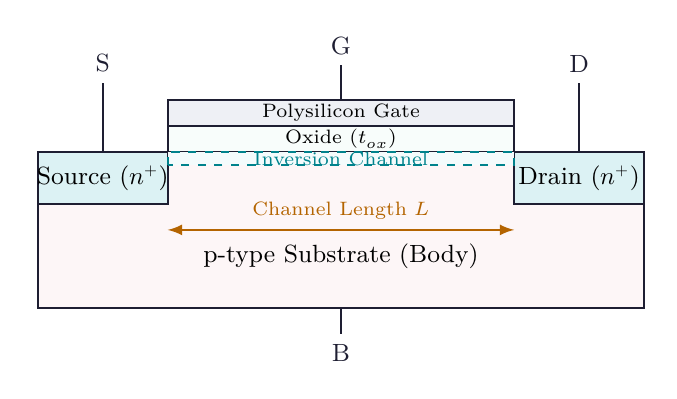
\begin{tikzpicture}[scale=1.1, thick, font=\small]
  % Substrate (P-type)
  \draw[draw=mydark, fill=hdrred!40] (-3.5, -1.8) rectangle (3.5, 0);
  \node at (0, -1.2) {p-type Substrate (Body)};
  
  % Source and Drain (N+ regions)
  \draw[draw=mydark, fill=hdrteal] (-3.5, -0.6) rectangle (-2.0, 0);
  \node at (-2.75, -0.3) {Source ($n^+$)};
  \draw[draw=mydark, fill=hdrteal] (2.0, -0.6) rectangle (3.5, 0);
  \node at (2.75, -0.3) {Drain ($n^+$)};
  
  % Gate Oxide
  \draw[draw=mydark, fill=hdrgreen!20] (-2.0, 0) rectangle (2.0, 0.3);
  \node[font=\scriptsize] at (0, 0.15) {Oxide ($t_{ox}$)};
  
  % Gate electrode
  \draw[draw=mydark, fill=hdrgray] (-2.0, 0.3) rectangle (2.0, 0.6);
  \node[font=\scriptsize] at (0, 0.45) {Polysilicon Gate};
  
  % Inversion channel
  \draw[draw=myteal, fill=hdrteal!30, dashed] (-2.0, -0.15) rectangle (2.0, 0);
  \node[font=\scriptsize, color=myteal] at (0, -0.08) {Inversion Channel};
  
  % Terminals and contacts
  \draw[line] (-2.75, 0) -- (-2.75, 0.8) node[above] {S};
  \draw[line] (0, 0.6) -- (0, 1.0) node[above] {G};
  \draw[line] (2.75, 0) -- (2.75, 0.8) node[above] {D};
  \draw[line] (0, -1.8) -- (0, -2.1) node[below] {B};
  
  % Dimension indicators
  \draw[latex-latex, color=myamber] (-2.0, -0.9) -- node[above, font=\scriptsize] {Channel Length $L$} (2.0, -0.9);
\end{tikzpicture}
\end{tcolorbox}

\subsection{Linear Region Derivation}
Let the coordinate along the channel be $y$, where $y = 0$ at the source and $y = L$ at the drain. Let $V(y)$ be the channel potential at position $y$.
The local mobile inversion charge density per unit area $Q_I(y)$ is:
\begin{equation}
  Q_I(y) = -C_{ox} \left[ V_{GS} - V(y) - V_{th} \right]
\end{equation}
The drift current in the channel is driven by the longitudinal electric field $E_y = -dV(y)/dy$. The drain current $I_D$ at any point $y$ is:
\begin{equation}
  I_D = W \cdot Q_I(y) \cdot v_y(y)
\end{equation}
where $W$ is the channel width, and $v_y(y)$ is the drift velocity of electrons: $v_y(y) = -\mu_n E_y(y) = \mu_n \frac{dV(y)}{dy}$.
Substituting the expressions:
\begin{equation}
  I_D = W \cdot \left( -C_{ox} \left[ V_{GS} - V(y) - V_{th} \right] \right) \cdot \left( -\mu_n \frac{dV(y)}{dy} \right)
\end{equation}
\begin{equation}
  I_D = \mu_n C_{ox} W \left[ V_{GS} - V(y) - V_{th} \right] \frac{dV(y)}{dy}
\end{equation}
Rearranging terms:
\begin{equation}
  I_D \cdot dy = \mu_n C_{ox} W \left[ V_{GS} - V_{th} - V(y) \right] dV(y)
\end{equation}
Integrating along the channel length from the source ($y=0, V(0)=0$) to the drain ($y=L, V(L)=V_{DS}$):
\begin{equation}
  \int_{0}^{L} I_D \, dy = \mu_n C_{ox} W \int_{0}^{V_{DS}} \left[ V_{GS} - V_{th} - V \right] dV
\end{equation}
Since $I_D$ is constant throughout the channel:
\begin{equation}
  I_D \cdot L = \mu_n C_{ox} W \left[ (V_{GS} - V_{th})V - \frac{V^2}{2} \right]_{0}^{V_{DS}}
\end{equation}
\begin{equation}
  I_D = \mu_n C_{ox} \frac{W}{L} \left[ (V_{GS} - V_{th})V_{DS} - \frac{V_{DS}^2}{2} \right]
\end{equation}
This is the \textbf{MOSFET Linear Region Current Equation} (valid for $V_{DS} < V_{GS} - V_{th}$).

\subsection{Saturation Region Derivation}
As $V_{DS}$ increases, the channel charge density at the drain end drops to zero when $V_{DS} = V_{GS} - V_{th}$. This condition is called \textbf{pinch-off}.
The saturation current $I_{D,\text{sat}}$ remains constant with further increases in $V_{DS}$. Substituting the pinch-off voltage $V_{DS} = V_{GS} - V_{th}$ into the linear current equation:
\begin{equation}
  I_{D,\text{sat}} = \mu_n C_{ox} \frac{W}{L} \left[ (V_{GS} - V_{th})(V_{GS} - V_{th}) - \frac{(V_{GS} - V_{th})^2}{2} \right]
\end{equation}
\begin{equation}
  I_{D,\text{sat}} = \frac{1}{2} \mu_n C_{ox} \frac{W}{L} \left( V_{GS} - V_{th} \right)^2
\end{equation}
This is the \textbf{MOSFET Saturation Region Current Equation} (valid for $V_{DS} \ge V_{GS} - V_{th}$).

\section{MOSFET Scaling Principles}

Scaling refers to reducing the physical dimensions of the MOSFET (channel length $L$, width $W$, gate oxide thickness $t_{ox}$) by a factor of $\beta > 1$ to increase packing density and speed.

\subsection{Types of Scaling}
\begin{itemize}[leftmargin=*, itemsep=3.5pt]
  \item \textbf{Constant-Field Scaling (Full Scaling):} All physical dimensions ($W, L, t_{ox}$) and voltages ($V_{DD}, V_{th}$) are scaled down by the factor $1/\beta$. This keeps the internal electric fields constant, preventing breakdown.
  \item \textbf{Constant-Voltage Scaling:} Only physical dimensions are scaled down by $1/\beta$, while the supply voltage $V_{DD}$ remains unchanged. This preserves system compatibility with older circuits (e.g. 5V logic) but leads to very high electric fields inside the chip.
\end{itemize}

\subsection{Scaling Factors Summary}
The table below summarizes how physical parameters scale under both scaling paradigms:

\begin{tcolorbox}[tikzbox, title={Comparison of Scaling Paradigms}]
\renewcommand{\arraystretch}{1.4}
\par\noindent
\begin{tabularx}{\linewidth}{|B{3.2cm}|>{\small\centering\arraybackslash}X|>{\small\centering\arraybackslash}X|}
\hline
\textbf{Parameter} & \textbf{\color{myred}Constant-Field} & \textbf{\color{myteal}Constant-Voltage} \\
\hline
\textbf{Dimensions ($W, L, t_{ox}$)} & $1/\beta$ & $1/\beta$ \\
\hline
\textbf{Voltages ($V_{DD}, V_{th}$)} & $1/\beta$ & $1$ \\
\hline
\textbf{Electric Field ($E$)} & $1$ & $\beta$ \\
\hline
\textbf{Capacitance ($C_{ox}$)} & $\beta$ & $\beta$ \\
\hline
\textbf{Drain Current ($I_D$)} & $1/\beta$ & $\beta$ \\
\hline
\textbf{Gate Delay ($\tau$)} & $1/\beta$ & $1/\beta^2$ \\
\hline
\textbf{Power Dissipation ($P$)} & $1/\beta^2$ & $\beta$ \\
\hline
\textbf{Power Density ($P/\text{Area}$)} & $1$ & $\beta^3$ \\
\hline
\end{tabularx}
\end{tcolorbox}
> [!WARNING]
> Under Constant-Voltage scaling, the power density increases by $\beta^3$. This causes massive heat dissipation issues in sub-micron chips, making Constant-Field (or hybrid) scaling mandatory for modern deep sub-micron VLSI designs.

\newpage
% ===============================================================================
% MANDATORY QUICK REVISION PAGE
% ===============================================================================
\begin{center}
  {\large\bfseries\color{myred} Quick Revision --- Module 2}\\[3pt]
  {\small\color{mydark} MOSFET Current Derivation \& Scaling $|$ PE-EC603C}
\end{center}
\noindent{\color{myred}\rule{\linewidth}{1.2pt}}
\vspace{4pt}

\begin{tcolorbox}[formulabox, title={\textbf{Key Module 2 Formulas}}]
$$\text{Linear Current:} \quad I_D = \mu_n C_{ox} \frac{W}{L} \left[ (V_{GS} - V_{th})V_{DS} - \frac{V_{DS}^2}{2} \right]$$
$$\text{Saturation Current:} \quad I_{D,\text{sat}} = \frac{1}{2} \mu_n C_{ox} \frac{W}{L} (V_{GS} - V_{th})^2 \left( 1 + \lambda V_{DS} \right)$$
$$\text{Pinch-off Condition:} \quad V_{DS,\text{sat}} = V_{GS} - V_{th} \qquad C_{ox} = \frac{\epsilon_{ox}}{t_{ox}}$$
\end{tcolorbox}

\begin{tcolorbox}[defbox, title={\textbf{One-Line Definitions}}]
\begin{itemize}[leftmargin=*, itemsep=2.5pt, topsep=0pt]
  \item \textbf{GCA:} Approximation assuming channel potential variations are much slower than gate oxide potential drops.
  \item \textbf{Pinch-off:} Condition where the inversion channel charge vanishes at the drain end ($V_{DS} = V_{GS} - V_{th}$).
  \item \textbf{Constant-Field Scaling:} Scaling method where dimensions and voltages are reduced by $\beta$ to keep internal fields constant.
  \item \textbf{Constant-Voltage Scaling:} Scaling method where dimensions are reduced by $\beta$ while voltages remain constant.
  \item \textbf{Subthreshold Current:} Leakage current that flows from drain to source even when $V_{GS} < V_{th}$.
  \item \textbf{Drift Velocity:} Average velocity attained by charged particles (electrons) in a material due to an electric field.
\end{itemize}
\end{tcolorbox}

\begin{tcolorbox}[exambox, title={\textbf{Frequently Asked / Viva Questions}}]
\begin{enumerate}[topsep=0pt, label=\textbf{Q\arabic*.}, itemsep=5pt]
  \item \Q{State the Gradual Channel Approximation (GCA) and its physical validity.}
    GCA assumes the longitudinal field along the channel $E_y = dV/dy$ changes very slowly compared to the vertical field $E_x$ across the oxide. It is highly valid for long-channel devices ($L \gg t_{ox}$), but breaks down in short-channel devices where $E_y$ is extremely high.
  \item \Q{Derive the drain current equation for a MOSFET operating in the linear region.}
    Starting with charge density $Q_I(y) = -C_{ox}(V_{GS} - V(y) - V_{th})$ and current $I_D = W Q_I(y) \mu_n (dV/dy)$, we integrate from $y=0$ to $L$ and $V=0$ to $V_{DS}$ to obtain the linear equation: $I_D = \mu_n C_{ox} \frac{W}{L} [(V_{GS} - V_{th})V_{DS} - V_{DS}^2 / 2]$.
  \item \Q{Explain the concept of channel pinch-off.}
    Pinch-off occurs when the voltage difference between the gate and the channel at the drain end falls below the threshold voltage, i.e., $V_{GD} = V_{GS} - V_{DS} = V_{th}$. At this point, the local inversion charge density at the drain becomes zero, and the current saturates.
  \item \Q{Why does Constant-Voltage scaling lead to reliability issues in sub-micron devices?}
    Because the physical dimensions ($L, t_{ox}$) are scaled down by $1/\beta$ while supply voltage stays constant, the internal electric fields increase by a factor of $\beta$. This causes oxide breakdown, hot-carrier injection, and velocity saturation.
  \item \Q{A MOSFET has $W = 10\,\mu\text{m}$, $L = 1\,\mu\text{m}$, $\mu_n C_{ox} = 100\,\mu\text{A/V}^2$, and $V_{th} = 0.8\,\text{V}$. Find $I_D$ at $V_{GS} = 2.0\,\text{V}$ and $V_{DS} = 0.5\,\text{V}$.}\\
    Here $V_{GS} - V_{th} = 2.0 - 0.8 = 1.2\,\text{V}$. Since $V_{DS} = 0.5\,\text{V} < 1.2\,\text{V}$, the device is in the linear region.\par
    $I_D = 100 \times 10 \left[ (1.2)(0.5) - 0.25/2 \right] = 1000 \left[ 0.6 - 0.125 \right] = 475\,\mu\text{A}$.
  \item \Q{Calculate the saturation current $I_{D,\text{sat}}$ for the same device ($V_{GS} = 2.0\,\text{V}, V_{DS} = 1.5\,\text{V}$).}\\
    Since $V_{DS} = 1.5\,\text{V} > 1.2\,\text{V}$, the device is in saturation.\par
    $I_{D,\text{sat}} = \frac{1}{2} \mu_n C_{ox} \frac{W}{L} (V_{GS} - V_{th})^2 = \frac{1}{2} \cdot 100 \cdot 10 \cdot (1.2)^2 = 500 \cdot 1.44 = 720\,\mu\text{A}$.
  \item \Q{Why does power density remain constant under constant-field scaling?}
    Under constant-field scaling, the power $P$ scales by $1/\beta^2$ and the chip area ($W \times L$) scales by $1/\beta^2$. Therefore, the ratio $P/\text{Area}$ scales by $(1/\beta^2)/(1/\beta^2) = 1$, keeping the thermal density constant.
  \item \Q{Derive the scaling factor of gate delay $\tau$ in constant-field scaling.}
    Gate delay is $\tau = \frac{C \cdot V}{I}$. Capacitance $C \propto W \cdot L / t_{ox}$ scales by $1/\beta$, voltage $V$ scales by $1/\beta$, and current $I$ scales by $1/\beta$. Thus, $\tau$ scales by $\frac{(1/\beta) \cdot (1/\beta)}{1/\beta} = 1/\beta$ (speed increases by $\beta$).
  \item \Q{What is the effect of channel length modulation on the saturation drain current?}
    It adds a term $(1 + \lambda V_{DS})$ to the saturation current equation. This represents the fact that after pinch-off, the effective channel length shortens as $V_{DS}$ increases, causing a small, linear increase in current rather than a flat saturation.
  \item \Q{Why is electron mobility ($\mu_n$) higher than hole mobility ($\mu_p$)?}
    Electrons reside in the conduction band where they have lower effective mass and experience less lattice scattering than holes, which move through the valence band by bond-breaking. This makes $\mu_n \approx 2.5$ to $3$ times higher than $\mu_p$.
\end{enumerate}
\end{tcolorbox}

\end{document}
